\documentclass[]{tufte-handout}

% ams
\usepackage{amssymb,amsmath}

\usepackage{ifxetex,ifluatex}
\usepackage{fixltx2e} % provides \textsubscript
\ifnum 0\ifxetex 1\fi\ifluatex 1\fi=0 % if pdftex
  \usepackage[T1]{fontenc}
  \usepackage[utf8]{inputenc}
\else % if luatex or xelatex
  \makeatletter
  \@ifpackageloaded{fontspec}{}{\usepackage{fontspec}}
  \makeatother
  \defaultfontfeatures{Ligatures=TeX,Scale=MatchLowercase}
  \makeatletter
  \@ifpackageloaded{soul}{
     \renewcommand\allcapsspacing[1]{{\addfontfeature{LetterSpace=15}#1}}
     \renewcommand\smallcapsspacing[1]{{\addfontfeature{LetterSpace=10}#1}}
   }{}
  \makeatother

\fi

% graphix
\usepackage{graphicx}
\setkeys{Gin}{width=\linewidth,totalheight=\textheight,keepaspectratio}

% booktabs
\usepackage{booktabs}

% url
\usepackage{url}

% hyperref
\usepackage{hyperref}

% units.
\usepackage{units}


\setcounter{secnumdepth}{-1}

% citations


% pandoc syntax highlighting

% longtable

% multiplecol
\usepackage{multicol}

% strikeout
\usepackage[normalem]{ulem}

% morefloats
\usepackage{morefloats}


% tightlist macro required by pandoc >= 1.14
\providecommand{\tightlist}{%
  \setlength{\itemsep}{0pt}\setlength{\parskip}{0pt}}

% title / author / date
\title[Econometrics II]{Homework 3}
\author{Ulrich Atz}
\date{2021-04-20}

\usepackage{tcolorbox}
\usepackage{multirow}

\begin{document}

\maketitle




\hypertarget{problem-1-coding-exercise}{%
\subsection{Problem 1 (Coding
Exercise)}\label{problem-1-coding-exercise}}

Using the Lalonde dataset and the \textbf{cobalt} package finish the
exercise from the slides.

That is:

Consider three possible matching techniques

\begin{enumerate}
\item Caliper matching on a single variable (pick the best one)
\item 4 nearest neighbor matching.
\item Propensity Score matching using a logit
\item Propensity Score matching using a kernel
\end{enumerate}

For each matching approach:

\begin{itemize}
\item[a.] Create a balance table. For each pretreatment covariate, include comparisons for treated and untreated units in terms of the mean and standard deviation. Report a test, for each covariate, of the hypothesis that the difference in means between treatment conditions is zero.


```r
data("lalonde", package = "cobalt")
covs0 <- subset(lalonde, select = -c(treat, re78))
(tab <- bal.tab(covs0, treat = lalonde$treat, thresholds = c(m = 0.05)))
```

```
## Note: 's.d.denom' not specified; assuming pooled.
```

```
## Balance Measures
##                Type Diff.Un      M.Threshold.Un
## age         Contin. -0.2419 Not Balanced, >0.05
## educ        Contin.  0.0448     Balanced, <0.05
## race_black   Binary  0.6404 Not Balanced, >0.05
## race_hispan  Binary -0.0827 Not Balanced, >0.05
## race_white   Binary -0.5577 Not Balanced, >0.05
## married      Binary -0.3236 Not Balanced, >0.05
## nodegree     Binary  0.1114 Not Balanced, >0.05
## re74        Contin. -0.5958 Not Balanced, >0.05
## re75        Contin. -0.2870 Not Balanced, >0.05
## 
## Balance tally for mean differences
##                     count
## Balanced, <0.05         1
## Not Balanced, >0.05     8
## 
## Variable with the greatest mean difference
##    Variable Diff.Un      M.Threshold.Un
##  race_black  0.6404 Not Balanced, >0.05
## 
## Sample sizes
##     Control Treated
## All     429     185
```
From the unmatched balance measure, we observe that the continuous variable with the greatest mean difference is _re74_, income in 1974. We use it for caliper matching.


```r
m_res <- list()

# Caliper on 0.1 std. dev.
m_res[[1]] <- matchit(treat ~ re75, data = lalonde,
caliper = c(0.1))

# Four nearest neighbor matching
m_res[[2]] <- matchit(treat ~ age + educ + race + married +
                    nodegree + re74 + re75, data = lalonde,
                    method = "nearest", distance = "mahalanobis", ratio = 4)
```

```
## Warning: Not all treated units will get 4 matches.
```

```r
# Propensity Score matching using a logit
m_res[[3]] <- matchit(treat ~ age + educ + race + married +
                    nodegree + re74 + re75, data = lalonde,
                    method = "nearest", distance = "glm", link = "logit")

# Propensity Score matching using a kernel
# Implement custom version?
m_res[[4]] <- matchit(treat ~ age + educ + race + married +
                   nodegree + re74 + re75, data = lalonde,
                   distance = "glm", link = "logit")

m_res <- set_names(m_res, c("Caliper", "NN4", "PScore", "Kernel"))

# Tables
map(m_res, ~ bal.tab(., treat = lalonde$treat, thresholds = c(m = 0.05), addl = ~ age + educ + lalonde$race  + lalonde$married + lalonde$nodegree + re74))
```

```
## $Caliper
## Call
##  matchit(formula = treat ~ re75, data = lalonde, caliper = c(0.1))
## 
## Balance Measures
##                         Type Diff.Adj         M.Threshold
## distance            Distance   0.0014     Balanced, <0.05
## re75                 Contin.  -0.0010     Balanced, <0.05
## age                  Contin.  -0.3669 Not Balanced, >0.05
## educ                 Contin.  -0.0487     Balanced, <0.05
## lalonde$race_black    Binary   0.6141 Not Balanced, >0.05
## lalonde$race_hispan   Binary  -0.0652 Not Balanced, >0.05
## lalonde$race_white    Binary  -0.5489 Not Balanced, >0.05
## lalonde$married       Binary  -0.2935 Not Balanced, >0.05
## lalonde$nodegree      Binary   0.1413 Not Balanced, >0.05
## re74                 Contin.  -0.6265 Not Balanced, >0.05
## 
## Balance tally for mean differences
##                     count
## Balanced, <0.05         3
## Not Balanced, >0.05     7
## 
## Variable with the greatest mean difference
##  Variable Diff.Adj         M.Threshold
##      re74  -0.6265 Not Balanced, >0.05
## 
## Sample sizes
##           Control Treated
## All           429     185
## Matched       184     184
## Unmatched     245       1
## 
## $NN4
## Call
##  matchit(formula = treat ~ age + educ + race + married + nodegree + 
##     re74 + re75, data = lalonde, method = "nearest", distance = "mahalanobis", 
##     ratio = 4)
## 
## Balance Measures
##                Type Diff.Adj         M.Threshold
## age         Contin.  -0.2455 Not Balanced, >0.05
## educ        Contin.   0.0278     Balanced, <0.05
## race_black   Binary   0.6532 Not Balanced, >0.05
## race_hispan  Binary  -0.0793 Not Balanced, >0.05
## race_white   Binary  -0.5739 Not Balanced, >0.05
## married      Binary  -0.3351 Not Balanced, >0.05
## nodegree     Binary   0.1126 Not Balanced, >0.05
## re74        Contin.  -0.7320 Not Balanced, >0.05
## re75        Contin.  -0.3557 Not Balanced, >0.05
## 
## Balance tally for mean differences
##                     count
## Balanced, <0.05         1
## Not Balanced, >0.05     8
## 
## Variable with the greatest mean difference
##  Variable Diff.Adj         M.Threshold
##      re74   -0.732 Not Balanced, >0.05
## 
## Sample sizes
##                      Control Treated
## All                   429.       185
## Matched (ESS)         414.01     185
## Matched (Unweighted)  429.       185
## 
## $PScore
## Call
##  matchit(formula = treat ~ age + educ + race + married + nodegree + 
##     re74 + re75, data = lalonde, method = "nearest", distance = "glm", 
##     link = "logit")
## 
## Balance Measures
##                 Type Diff.Adj         M.Threshold
## distance    Distance   0.9739                    
## age          Contin.   0.0718 Not Balanced, >0.05
## educ         Contin.  -0.1290 Not Balanced, >0.05
## race_black    Binary   0.3730 Not Balanced, >0.05
## race_hispan   Binary  -0.1568 Not Balanced, >0.05
## race_white    Binary  -0.2162 Not Balanced, >0.05
## married       Binary  -0.0216     Balanced, <0.05
## nodegree      Binary   0.0703 Not Balanced, >0.05
## re74         Contin.  -0.0505 Not Balanced, >0.05
## re75         Contin.  -0.0257     Balanced, <0.05
## 
## Balance tally for mean differences
##                     count
## Balanced, <0.05         2
## Not Balanced, >0.05     7
## 
## Variable with the greatest mean difference
##    Variable Diff.Adj         M.Threshold
##  race_black    0.373 Not Balanced, >0.05
## 
## Sample sizes
##           Control Treated
## All           429     185
## Matched       185     185
## Unmatched     244       0
## 
## $Kernel
## Call
##  matchit(formula = treat ~ age + educ + race + married + nodegree + 
##     re74 + re75, data = lalonde, distance = "glm", link = "logit")
## 
## Balance Measures
##                 Type Diff.Adj         M.Threshold
## distance    Distance   0.9739                    
## age          Contin.   0.0718 Not Balanced, >0.05
## educ         Contin.  -0.1290 Not Balanced, >0.05
## race_black    Binary   0.3730 Not Balanced, >0.05
## race_hispan   Binary  -0.1568 Not Balanced, >0.05
## race_white    Binary  -0.2162 Not Balanced, >0.05
## married       Binary  -0.0216     Balanced, <0.05
## nodegree      Binary   0.0703 Not Balanced, >0.05
## re74         Contin.  -0.0505 Not Balanced, >0.05
## re75         Contin.  -0.0257     Balanced, <0.05
## 
## Balance tally for mean differences
##                     count
## Balanced, <0.05         2
## Not Balanced, >0.05     7
## 
## Variable with the greatest mean difference
##    Variable Diff.Adj         M.Threshold
##  race_black    0.373 Not Balanced, >0.05
## 
## Sample sizes
##           Control Treated
## All           429     185
## Matched       185     185
## Unmatched     244       0
```

\item[b.] For each covariate, plot its distribution under treatment and control


```r
# Plots, loop over models and vars
map(m_res, function(x) {
    map(names(x$X), ~ bal.plot(x, ., which = "both"))
    })
```

```
## $Caliper
## $Caliper[[1]]
```


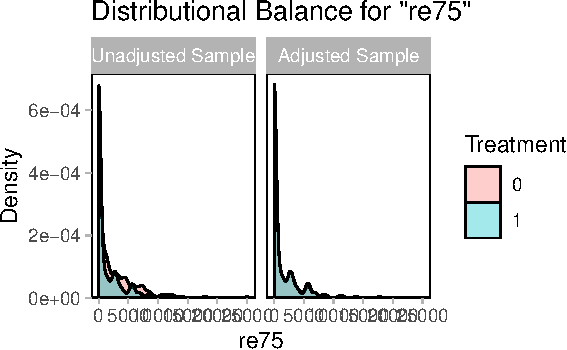
\includegraphics{assignment_3_treatment_files/figure-latex/unnamed-chunk-3-1} 

```
## 
## 
## $NN4
## $NN4[[1]]
```


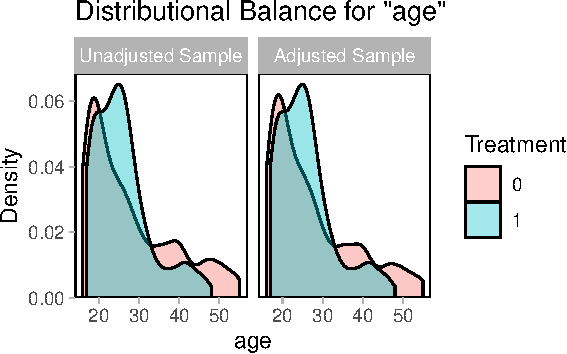
\includegraphics{assignment_3_treatment_files/figure-latex/unnamed-chunk-3-2} 

```
## 
## $NN4[[2]]
```


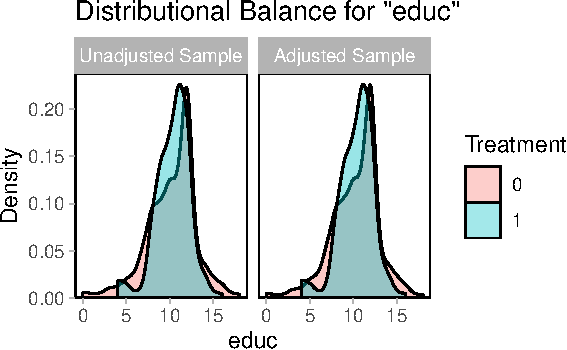
\includegraphics{assignment_3_treatment_files/figure-latex/unnamed-chunk-3-3} 

```
## 
## $NN4[[3]]
```


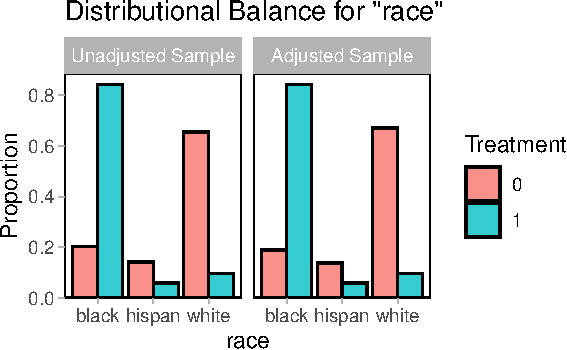
\includegraphics{assignment_3_treatment_files/figure-latex/unnamed-chunk-3-4} 

```
## 
## $NN4[[4]]
```


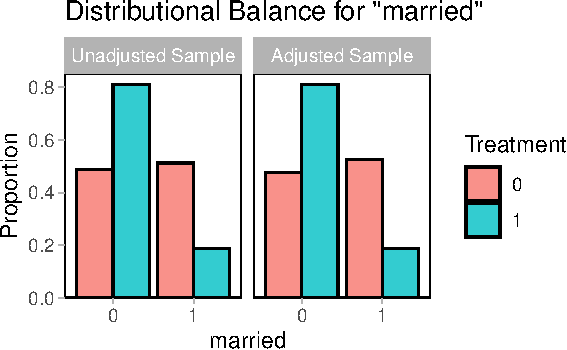
\includegraphics{assignment_3_treatment_files/figure-latex/unnamed-chunk-3-5} 

```
## 
## $NN4[[5]]
```


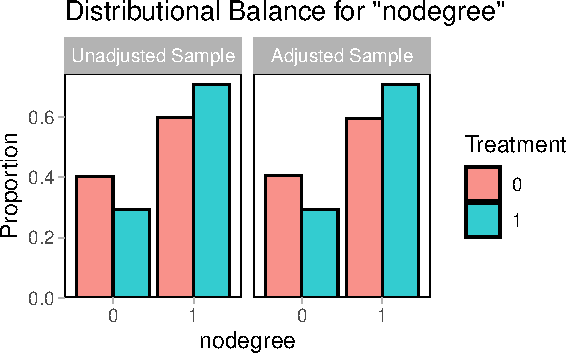
\includegraphics{assignment_3_treatment_files/figure-latex/unnamed-chunk-3-6} 

```
## 
## $NN4[[6]]
```


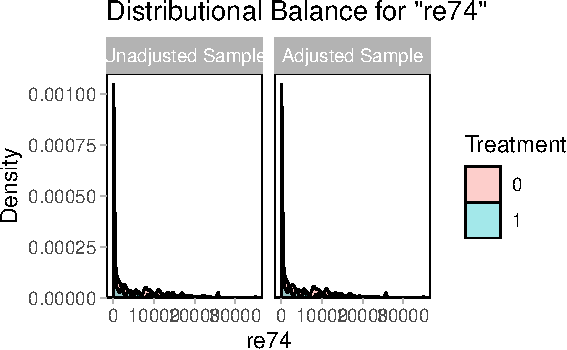
\includegraphics{assignment_3_treatment_files/figure-latex/unnamed-chunk-3-7} 

```
## 
## $NN4[[7]]
```


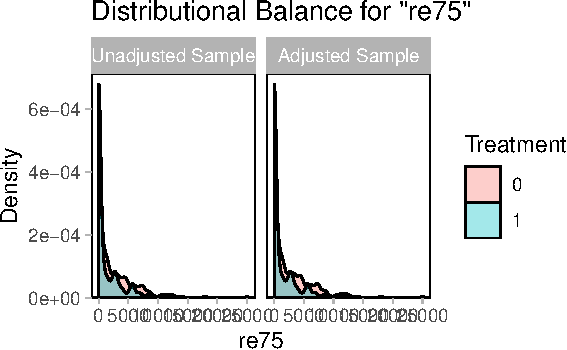
\includegraphics{assignment_3_treatment_files/figure-latex/unnamed-chunk-3-8} 

```
## 
## 
## $PScore
## $PScore[[1]]
```


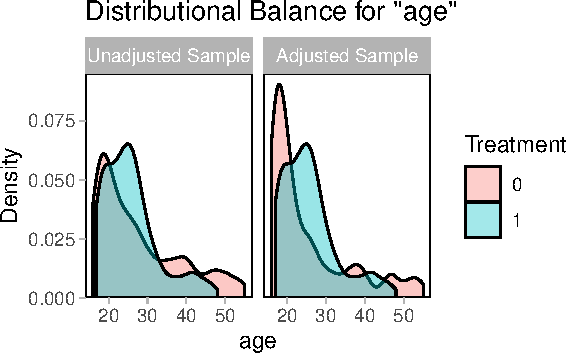
\includegraphics{assignment_3_treatment_files/figure-latex/unnamed-chunk-3-9} 

```
## 
## $PScore[[2]]
```


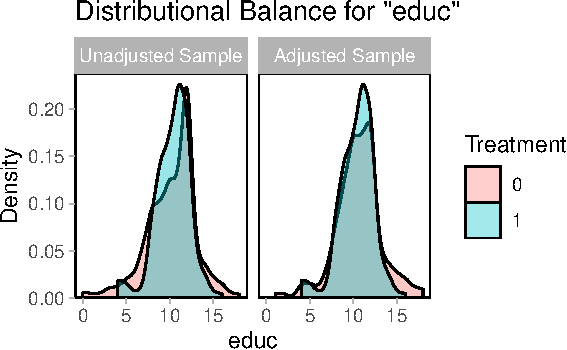
\includegraphics{assignment_3_treatment_files/figure-latex/unnamed-chunk-3-10} 

```
## 
## $PScore[[3]]
```


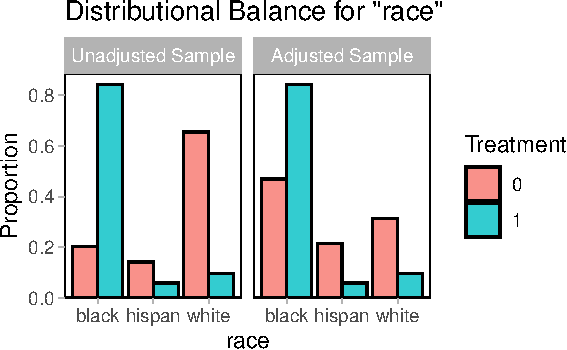
\includegraphics{assignment_3_treatment_files/figure-latex/unnamed-chunk-3-11} 

```
## 
## $PScore[[4]]
```


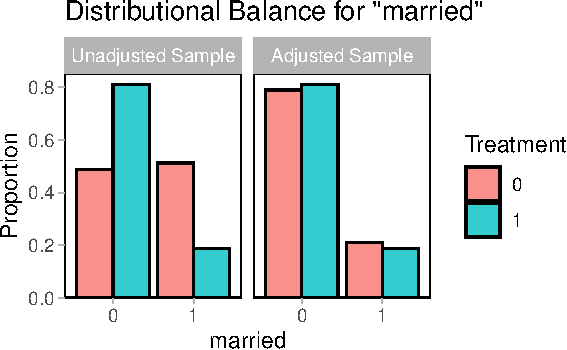
\includegraphics{assignment_3_treatment_files/figure-latex/unnamed-chunk-3-12} 

```
## 
## $PScore[[5]]
```


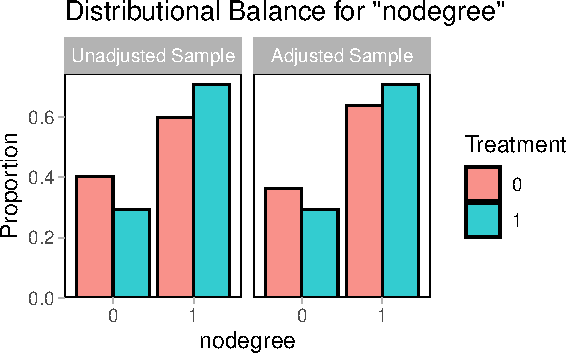
\includegraphics{assignment_3_treatment_files/figure-latex/unnamed-chunk-3-13} 

```
## 
## $PScore[[6]]
```


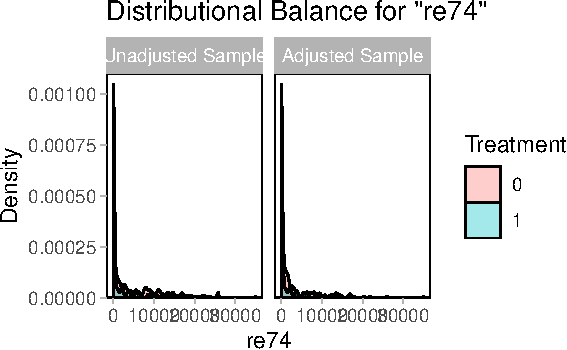
\includegraphics{assignment_3_treatment_files/figure-latex/unnamed-chunk-3-14} 

```
## 
## $PScore[[7]]
```


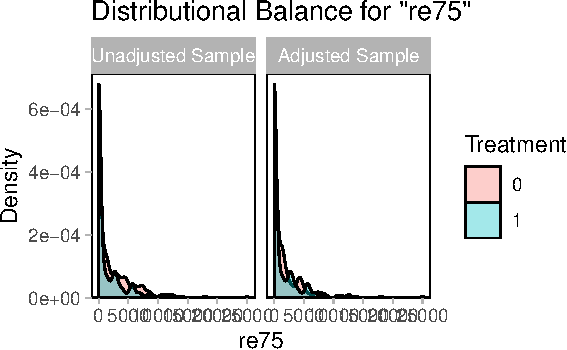
\includegraphics{assignment_3_treatment_files/figure-latex/unnamed-chunk-3-15} 

```
## 
## 
## $Kernel
## $Kernel[[1]]
```


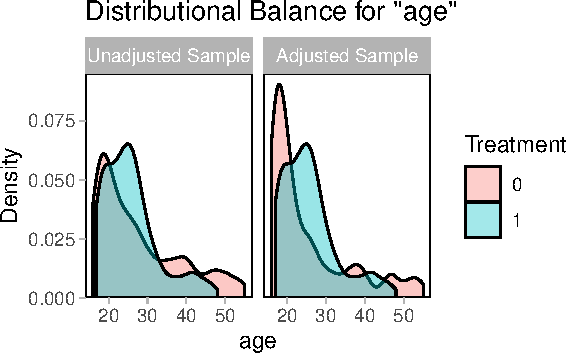
\includegraphics{assignment_3_treatment_files/figure-latex/unnamed-chunk-3-16} 

```
## 
## $Kernel[[2]]
```


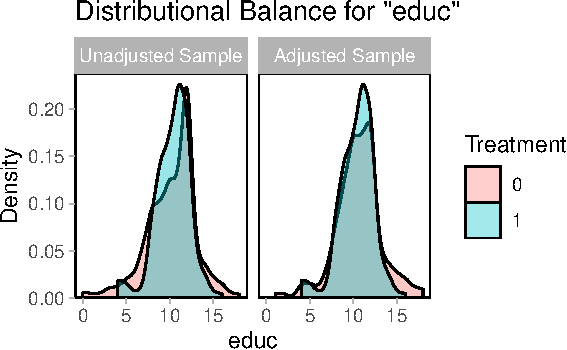
\includegraphics{assignment_3_treatment_files/figure-latex/unnamed-chunk-3-17} 

```
## 
## $Kernel[[3]]
```


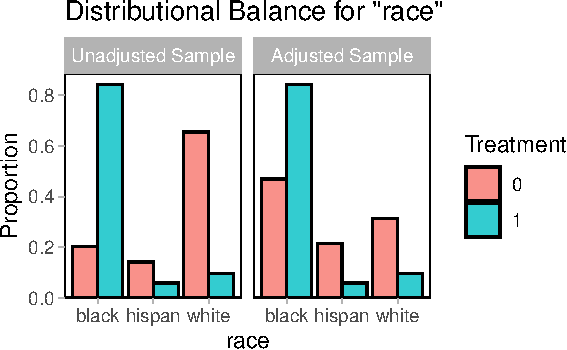
\includegraphics{assignment_3_treatment_files/figure-latex/unnamed-chunk-3-18} 

```
## 
## $Kernel[[4]]
```


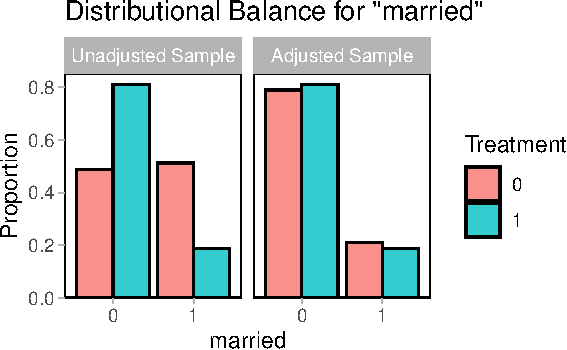
\includegraphics{assignment_3_treatment_files/figure-latex/unnamed-chunk-3-19} 

```
## 
## $Kernel[[5]]
```


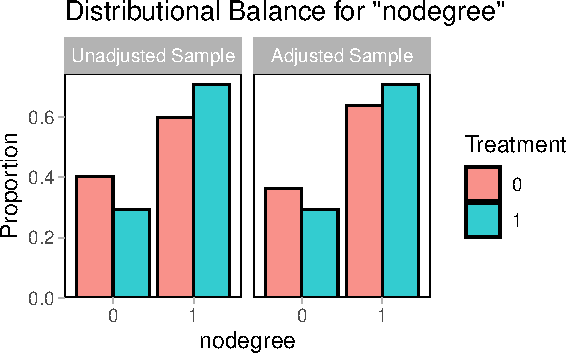
\includegraphics{assignment_3_treatment_files/figure-latex/unnamed-chunk-3-20} 

```
## 
## $Kernel[[6]]
```


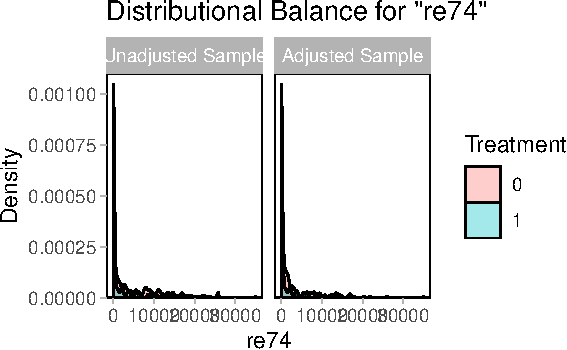
\includegraphics{assignment_3_treatment_files/figure-latex/unnamed-chunk-3-21} 

```
## 
## $Kernel[[7]]
```


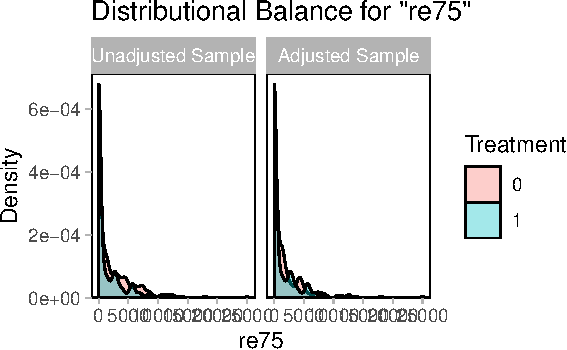
\includegraphics{assignment_3_treatment_files/figure-latex/unnamed-chunk-3-22} 

\item[c.] Estimate the ATT and/or ATE of participating in the job training program


```r
library(lmtest, quietly = T)
```

```
## 
## Attaching package: 'zoo'
```

```
## The following objects are masked from 'package:base':
## 
##     as.Date, as.Date.numeric
```

```r
library(sandwich, quietly = T)

map(m_res, function(x){
  md <- match.data(x)
  fit <- lm(re78 ~ treat, data = md, weights = weights)
  coeftest(fit, vcov. = vcovCL, cluster = ~subclass)
})
```

```
## $Caliper
## 
## t test of coefficients:
## 
##             Estimate Std. Error t value Pr(>|t|)    
## (Intercept)  6492.43     537.29 12.0836   <2e-16 ***
## treat        -131.51     798.65 -0.1647   0.8693    
## ---
## Signif. codes:  0 '***' 0.001 '**' 0.01 '*' 0.05 '.' 0.1 ' ' 1
## 
## 
## $NN4
## 
## t test of coefficients:
## 
##             Estimate Std. Error t value Pr(>|t|)    
## (Intercept)  7000.83     375.09 18.6641   <2e-16 ***
## treat        -651.68     663.55 -0.9821   0.3264    
## ---
## Signif. codes:  0 '***' 0.001 '**' 0.01 '*' 0.05 '.' 0.1 ' ' 1
## 
## 
## $PScore
## 
## t test of coefficients:
## 
##             Estimate Std. Error t value Pr(>|t|)    
## (Intercept)  5454.78     446.43 12.2187   <2e-16 ***
## treat         894.37     715.76  1.2495   0.2123    
## ---
## Signif. codes:  0 '***' 0.001 '**' 0.01 '*' 0.05 '.' 0.1 ' ' 1
## 
## 
## $Kernel
## 
## t test of coefficients:
## 
##             Estimate Std. Error t value Pr(>|t|)    
## (Intercept)  5454.78     446.43 12.2187   <2e-16 ***
## treat         894.37     715.76  1.2495   0.2123    
## ---
## Signif. codes:  0 '***' 0.001 '**' 0.01 '*' 0.05 '.' 0.1 ' ' 1
```
\item[d.] Can you estimate both ATE or ATT? Why or why not?

The ATT is the estimand we computed above. The ATE is a weighted average between the effect on the treated and the effect on the untreated.

$$ ATE = \pi \cdot ATT + (1-\pi) \cdot ATUT $$

Technically, the ATE is only available for methods that do not discard units. For example, if we do not find enough matches when estimating the ATUT because the control group is larger, we are in effect assuming a different target population. 

\end{itemize}

\hypertarget{problem-2-coding-exercise}{%
\subsection{Problem 2 (Coding
Exercise)}\label{problem-2-coding-exercise}}

The dataset for this exercise comes from a paper by Benjamin Olken
entitled ``Monitoring Corruption: Evidence from a Field Experiment in
Indoneisa''. The paper evaluates an attempt to reduce corruption in road
building in Indonesia. The treatment we focus on was ``accountability
meetings''. These meetings were held at a village level, and project
officials were probed to account for how they spent project funds.
Before construction began, residents in the treated villages were
encouraged to attend these meetings. The dataset is called
``olken.csv''.

The outcome we care about is \textbf{pct.missing}, the difference
between what officials claim they spent on road construction and an
independent measure of expenditures. Treatment is given by
\textbf{treat.invite} such that:

\begin{align*}
  \text{treat.invite} = 
    \begin{cases}
      1 &\mbox{ if village received intervention} \\
      0 &\mbox{ if village was control }
    \end{cases}
\end{align*}

We have the following four pre-treatment covariates:

\begin{itemize}
  \item[--] head.edu : the education of the village head
  \item[--] mosques : mosques per 1000 residents
  \item[--] pct.poor : the percentage of households below the poverty line
  \item[--] total.budget : the budget for each project
\end{itemize}

We now have the following questions:

\begin{itemize}

\item[a.] Create a balance table. For each pretreatment covariate, include comparisons for treated and untreated units in terms of the mean and standard deviation. Report a test, for each covariate, of the hypothesis that the difference in means between treatment conditions is zero.


```r
olken <- read_csv("data/olken.csv")
covs2 <- subset(olken, select = -c(treat.invite, pct.missing, id))
(tab2 <- bal.tab(covs2, treat = olken$treat.invite, thresholds = c(m = 0.05)))
```

```
## Balance Measures
##                 Type Diff.Un      M.Threshold.Un
## head.edu     Contin. -0.0137     Balanced, <0.05
## mosques      Contin. -0.0642 Not Balanced, >0.05
## pct.poor     Contin.  0.0482     Balanced, <0.05
## total.budget Contin. -0.0036     Balanced, <0.05
## 
## Balance tally for mean differences
##                     count
## Balanced, <0.05         3
## Not Balanced, >0.05     1
## 
## Variable with the greatest mean difference
##  Variable Diff.Un      M.Threshold.Un
##   mosques -0.0642 Not Balanced, >0.05
## 
## Sample sizes
##     Control Treated
## All     161     311
```


\item[b.] For each covariate, plot its distribution under treatment and control (either side-by-side using facetgrid or overlap).


```r
map(names(covs2), function(x){
    ggplot(olken, aes(x)) + 
      geom_density() +
      facet_wrap(~treat.invite)
    })
```

```
## [[1]]
```


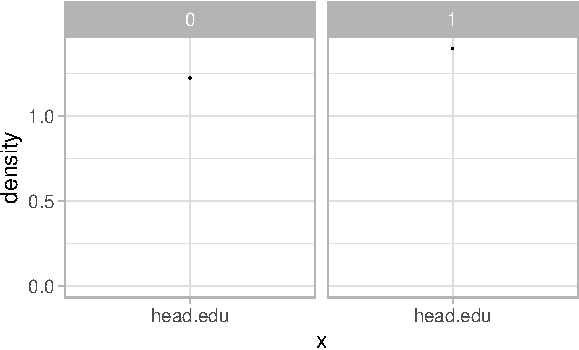
\includegraphics{assignment_3_treatment_files/figure-latex/unnamed-chunk-6-1} 

```
## 
## [[2]]
```


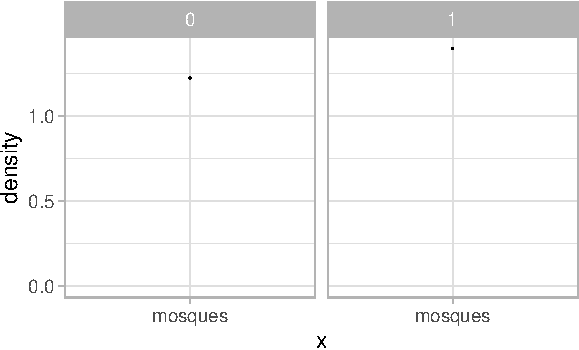
\includegraphics{assignment_3_treatment_files/figure-latex/unnamed-chunk-6-2} 

```
## 
## [[3]]
```


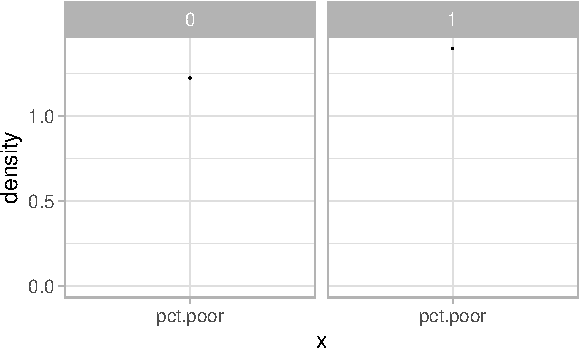
\includegraphics{assignment_3_treatment_files/figure-latex/unnamed-chunk-6-3} 

```
## 
## [[4]]
```


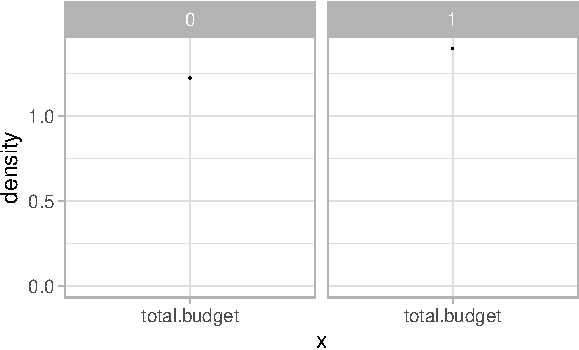
\includegraphics{assignment_3_treatment_files/figure-latex/unnamed-chunk-6-4} 

\item[c.] Given your answers to part a and b, do the villagers seem similar in their pre-treatment covariates?

\item[d.] Regress the treatment on the pre-treatment covariates. What do you conclude?

\item[e.] Using the difference-in-means estimator, estimate the ATE and its standard error.

\item[f.] Using a simple regression of outcomes on treatment, estimate the ATE and its standard error. Compare your answer in (f) to (e).

\item[g.] Using the same regression from part (f), include pre-treatment covariates in your regression equation (additively and linearly). Report estimates of treatment effects and its standard error. Do you expect (g) to differ from (f) and (e)? Explain your answer.

\end{itemize}

\hypertarget{problem-3-coding-exercise}{%
\subsection{Problem 3 (Coding
Exercise)}\label{problem-3-coding-exercise}}

We will be using a dataset that was simulated from real data. Oftentimes
due to privacy concerns researchers will provide simulated data from the
distribution of real data. The dataset you will be using are from a
tutoring program focused on math for 7th graders. The dataset is called
``tests\_Rd.csv''. The tutoring is the treatment variable,
\textbf{treat}. Tutoring was given to students based on a pretest score,
\textbf{pretest} thus the pretest score is the forcing variable.
Students that received less than 215 were given a tutor. Our outcome of
interest is the test score after tutoring, \textbf{posttest}.

We also have a series of control variables:

\begin{itemize}
  \item[--] age     : age of student as of September 2010
  \item[--] gender  : 1 if student's gender is male
  \item[--] frlunch : 1 if student is eligible a free lunch
  \item[--] esol    : 1 if student has english as a second language
  \item[--] white   : 1 if student's race/ethnicity is white
  \item[--] asian   : 1 if student's race/ethnicity is asian
  \item[--] black   : 1 if student's race/ethnicity is black
  \item[--] hispanic: 1 if student's race/ethnicity is hispanic
\end{itemize}

We ask you to answer the following questions:

\begin{enumerate}

\item[a.] We want you to first plot the graph that justifies a sharp RD design. Plot the treatment as a function of the forcing variable. What do you see?

\item[b.] We now want you to plot the graph that justifies our forcing variable. Plot the outcome as a function of the forcing variable. What do you see?

\item[c.]  Estimate the local average treatment effect (LATE) at the threshold using a linear model with common slopes for treated and control units (with no control variables). What are the additional assumptions required for this estimation strategy? Provide a plot of the post test scores (y-axis) and forcing variable (x-axis) in which you show the fitted curves and the underlying scatterplot of the data. Interpret your resulting estimate.

\item[d. ] Re-do c., but use the control variables that are provided in the dataset. Interpret any differences you see. 

\item[e. ] Use the rdd package in R to estimate the LATE at the threshold using a local linear regression with a triangular kernel. Note that the function RDestimate automatically uses the Imbens-Kalyanamaran optimal bandwidth calculation. Report your estimate for the LATE and an estimate of uncertainty.

\item[f. ] How do the estimates of the LATE at the threshold differ based on your results from parts (b) to (e)? In other words, how robust are the results to different specifications of the regression? What other types of robustness checks might be appropriate?
\end{enumerate}

We are now going to do a series of robustness checks:

\begin{enumerate}
\item[h. ] Plot the age variable as a function of the forcing variable. What should this graph look like for our RDD to be a valid design? What do you see? How does this relate to the covariate balance exercise we did in Problem 1?

\item[i. ] One type of placebo test is to pick arbitrary cutoffs of your forcing variable and estimate LATE's for those cutoffs. Pick 10 cutoffs and report the average LATE across those cutoffs. Defining $\hat{\tau}$ as your average LATEs, what should the null hypothesis on the population counterpart of this estimator be for our design to be valid. Feel free to use which specification you want for estimating LATE, but please specify it.

\item[k. ] An issue with RD designs is manipulation, or sorting around the cutoff point. To assess this, plot a histogram of the forcing variable, drawing a line at the cutoff point. What would sorting around the cutoff point look like? What do you see? 


\end{enumerate}



\end{document}
